\documentclass[11pt]{article}
\title{How the Codynamic Book Machine Works}
\author{Arthur Petron}
\usepackage[margin=1in]{geometry}
\usepackage{graphicx}
\usepackage{amsmath,amssymb,mathtools}
\usepackage{tikz}
\usetikzlibrary{positioning,arrows.meta}
\usepackage{hyperref}
\graphicspath{{media/}{media/diagrams/}{images/}{artwork/}}

\begin{document}

\section*{Agent Roles}

The Codynamic Book Machine divides authoring work among a small set of specialized agents, each with a narrow responsibility and a clear handoff boundary. That division is not incidental: it is the mechanism that keeps outline intent, prose generation, editorial maintenance, references, diagrams, design, and compilation aligned as the manuscript evolves.

At the top of the runtime is the hypervisor, which supervises the whole project and coordinates work across agents. It receives high-level intent, starts section work, and escalates cross-cutting issues when a local fix is not enough. In practice, the hypervisor acts as the system's orchestration layer: it knows which section is being worked on, which tasks are pending, and when a callback or repair request should be routed to a specialist rather than handled inline.

The outlining and intake functions translate author intent into a structured work object. They are responsible for turning a topic, audience, and desired scope into a canonical outline that can be decomposed into chapters, sections, and subsections. Once the outline exists, it becomes the shared reference point for all downstream agents. Section agents do not invent the book's structure; they interpret and realize the structure that the outline already declares.

Section drafting is the responsibility of the section agents. Each section agent owns one section payload at a time and writes the \LaTeX{} body for that section only. Its job is to convert outline intent, imported source material, and runtime feedback into coherent prose that fits the surrounding chapter. Section agents also participate in the system's coordination protocol: they inspect their own section in context, choose among queued tasks, respond to callbacks, and revise their text when the gardener, references agent, diagram agent, or design agent identifies a needed change.

The gardener is the editorial maintenance agent. Rather than waiting for a human editor to notice drift, the gardener continuously checks the manuscript for repeated claims, thin transitions, missing definitions, unsupported assertions, and inconsistencies between a section and its neighbors. When it finds a local issue, it can request a targeted revision from the relevant section agent. When it finds a broader mismatch, it escalates the problem so the hypervisor can coordinate a wider repair. In this way, gardening functions as proactive editorial control rather than passive validation.

Reference support is handled by the references agent. It owns the shared bibliography and the canonical record of registered citation keys, which means section agents do not edit the bibliography directly. Instead, when a section needs support for a claim or a definition that is not already registered, the section agent must request research or hand off the missing support to the references agent. This separation keeps citation management centralized and prevents ad hoc bibliography drift. Section agents are expected to cite only registered keys, and to verify that a key exists before using it in the section text.

Diagram work is routed through the diagram agent. Section agents may propose diagrams when a visual would materially improve the explanation, but they do not fabricate diagram assets or paths. Instead, they send a structured request describing the section-specific concept that needs visualization, the purpose of the figure, and the relationships it should show. The diagram agent then creates the asset and returns a callback with the media path and inclusion hint. This keeps visual design distinct from prose drafting while still allowing the section to benefit from targeted illustrations.

Document design is a separate concern from section authorship. The design agent reviews the compiled manuscript as a document, not as isolated sections, and can flag layout, readability, or presentation issues that are better addressed at the document level than in a single section payload. That distinction matters because some problems are local to a paragraph, while others concern the overall shape of the paper, the balance of sections, or the consistency of the final artifact.

Finally, assembly turns the distributed work of the agents into a compiled paper. The assembler consumes the section payloads, bibliography, media assets, and build configuration, then produces the durable outputs that readers actually see. Assembly is the point at which the system's separate artifacts become a single document, but it is not the point at which authorship ends. If compilation exposes an error or a mismatch, the result is routed back into the agent workflow as a repair task, preserving the same durable, inspectable loop that governs drafting and revision.

Taken together, these roles form a layered division of labor: hypervision coordinates, outlining structures, section agents draft, gardening maintains coherence, references support claims, diagrams externalize relationships, design shapes presentation, and assembly produces the final artifact. The system's central design choice is that each responsibility has a specialist owner and a visible handoff, so the manuscript can evolve without losing track of who is responsible for what.

\begin{figure}[htbp]
\centering
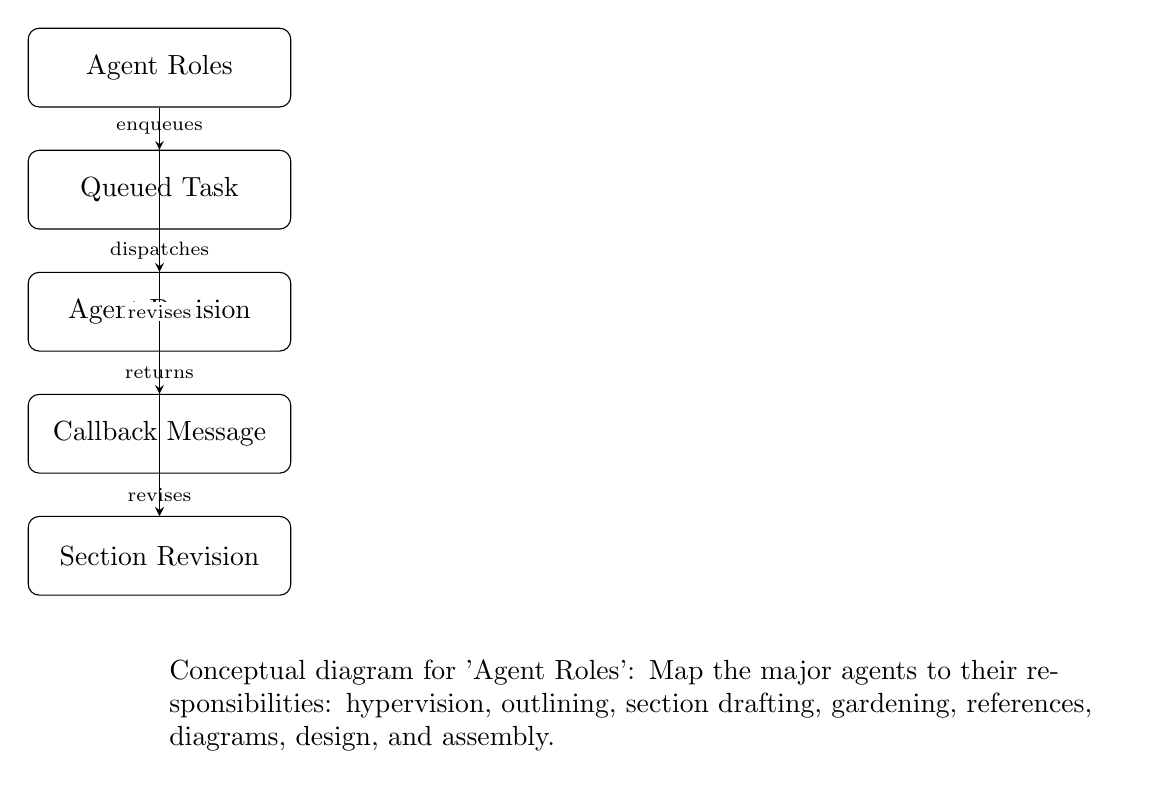
\begin{tikzpicture}[>=stealth, node distance=2.2cm,
  concept/.style={draw, rounded corners, align=center, text width=3.1cm, minimum height=1cm},
  relation/.style={font=\scriptsize, fill=white, inner sep=1pt}]
\node[concept] (n1) at (0,0.0) {Agent Roles};
\node[concept] (n2) at (0,-1.55) {Queued Task};
\node[concept] (n3) at (0,-3.1) {Agent Decision};
\node[concept] (n4) at (0,-4.65) {Callback Message};
\node[concept] (n5) at (0,-6.2) {Section Revision};
\draw[->] (n1) -- node[relation] {enqueues} (n2);
\draw[->] (n2) -- node[relation] {dispatches} (n3);
\draw[->] (n3) -- node[relation] {returns} (n4);
\draw[->] (n4) -- node[relation] {revises} (n5);
\draw[->] (n1) -- node[relation] {revises} (n5);
\node[align=left, text width=12cm, anchor=north west] at (0,-7.4) {Conceptual diagram for 'Agent Roles': Map the major agents to their responsibilities: hypervision, outlining, section drafting, gardening, references, diagrams, design, and assembly.};
\end{tikzpicture}

\caption{Conceptual diagram for ``Agent Roles'': Map the major agents to their responsibilities: hypervision, outlining, section drafting, gardening, references, diagrams, design, and assembly.}
\end{figure}


\end{document}
